\documentclass[11pt]{memoir}

% need it in .docx form? no problem!
% pandoc -s chapter-2.tex -o chapter-2.docx --bibliography="chapter-2.bib"; mv chapter-2.docx ~/Desktop

\usepackage{import}
\import{../}{gov-style}
% \addbibresource{../thesis.bib}

\begin{document}
\begin{refsegment}

% \section*{Thesis so far}
% \begin{em}
% In this thesis, I seek to understand why nation-states (and the United States in particular) do not respond more harshly to cyber-espionage. While the US takes the appropriate steps to prevent digital invasions, it appears that they don't punish states diplomatically for hacking into our systems and attempting to steal state secrets. I theorize that this puzzling response to cyber-attacks can be explained by espionage norms that formed during the Cold War---norms that prescribe a state will never extend the diplomatic consequences of an espionage attempt beyond the countermeasures necessary to prevent it. To make this connection, I will demonstrate the various forms in which this norm existed during the Cold War, then analyze how it influences our cybersecurity policy today.

% To prove that this norm exists, each of the next three chapters will examine a different vector of espionage between the United States and the USSR: aerial reconnaissance, human intelligence, and other technological intelligence advancements like satellites. In each chapter, I will present a timeline of how that espionage method was used in the Cold War, investigate instances in which its use provoked the most severe diplomatic consequences, and argue that those consequences demonstrate an upper limit on the severity with which a state will respond to uncovering attempted espionage. In this chapter, we take a look at aerial reconnaissance.
% \end{em}


\section{Introduction}
Planes have been used as a reconnaissance tool for almost as long as they have existed at all. According to \emph{The New York Times}, the very first reconnaissance flight was in 1911, only eight years after Kitty Hawk, when ``Lieut. Piazzi today, for the first time in the history of warfare, made from this place an aerial reconnaissance against a hostile power'' surveilling the Turkish Infantry near Tripoli.\footcite{special_cable_to_the_new_york_times_air_1911} The ability to fly over an enemy's position to gain intelligence about their movements---in a craft orders of magnitude more versatile than a balloon---was so obviously valuable that countermeasures quickly followed. Early aerial dogfighting famously took the form of pilots firing handguns at each other out of open cockpits in mid-air (emphasis on attempted), but by the time of the First World War, planes were already outfitted with synchronized machine guns and ground regiments equipped with anti-aircraft weaponry. Crucial information about military movements was going to come at a cost.

Even though these aircraft were performing vital intelligence-gathering functions, that did not make them spy planes. Aerial reconnaissance first appeared in the press in 1911, but the term ``spy plane'' appeared in the pages of \emph{The New York Times} just once before 1960.\footnote{According to my search of the archives. The instance mentioned here was in 1944, when the AP wrote that ``Germans tried to probe the secrets of the gathering Allied storm by E-boat patrol dashes [...] and by spy-plane coastal raids.''(\cite{the_associated_press_britons_1944}) In context of the article, though, it's clear that they are referring to military aerial reconnaissance, especially since it was written during the Second World War. This is a marked difference from a plane created for intelligence gathering purposes, which would come later.} The image of a spy plane crashed into the public consciousness that year as Gary Powers crawled out of a U-2 class aircraft over Soviet Russia. The downed craft was clearly not a generic fighter plane that had flown too close to the border, and it suddenly became necessary to categorize this new instrument, flying at previously unheard-of altitudes, purpose-built for clandestine photography. The United States first tried to claim that the lost plane was a ``weather craft.''\footcite{caruthers_soviet_1960} When that cover didn't hold up, a new story was born. The diplomatic fallout of the U-2 shootdown, which threatened to torpedo an upcoming NATO-Warsaw summit, had become the ``spy-plane case.''\footcite[This is the second time that ``spy plane'' as a term of art appeared in \emph{The New York Times}. There would be many more.]{reston_allies_1960}

I emphasize the linguistic distinction between a military plane used for reconnaissance and a ``spy plane'' because that distinction has a major impact on how the flight is perceived and what diplomatic repercussions might result when it is caught.\footnote{That is not to say there is a hard boundary between military and non-military intelligence, either in purpose or collection. The overlap between military and civilian intelligence agencies---especially in the United States---is considerable. The Air Force was deeply involved with the U-2 Project, for example, even though it was technically under the jurisdiction of the CIA. The aerial photographs taken by U-2 missions were used to inform both military and civilian operations.} A military fight carries with it the implications of combat, aggression, and the possible prelude to an attack. A spy flight is instead a tool of civilian intelligence, whose purposes are often frustrated but never quite discouraged. The creation of the U-2 plane---a craft exclusively designed for civilian intelligence---is a pivotal moment in the history of espionage because the U-2 is the physical embodiment of the norms it helped to define. Its \emph{raison d'\^etre} is an activity which is not permitted---or its altitude would be unnecessary---but its design makes clear that it only plans to observe.

\section{The Open Skies policy}
From the beginning of the Cold War, aerial intelligence played a crucial role in American foreign policy. The United States considered aerial surveillance so important that they were willing to allow the Soviets to do it to them in return. President Eisenhower formally proposed a mutual inspection regime called Open Skies to the Soviet Union as a means of reducing security tensions. In his prepared remarks at the Geneva Summit of 1955, Eisenhower laid out the following plan (emphasis mine):

\begin{quote}
\textbf{To give to each other a complete blueprint of our military establishments}, from beginning to end, from one end of our countries to the other, lay out the establishments and provide the blueprints to each other.
\newline

Next, to provide within our countries facilities for aerial photography to the other country---\textbf{we to provide you the facilities within our country, ample facilities for aerial reconnaissance}, where you can make all the pictures you choose and take them to your own country to study, you to provide exactly the same facilities for us and we to make these examinations, and by this step \textbf{to convince the world that we are providing as between ourselves against the possibility of great surprise attack}, thus lessening danger and relaxing tension.\footcite{eisenhower_president_1955}
\end{quote}

The UN-sponsored Geneva Summit, formally the \emph{Conference on the Peaceful Uses of Atomic Energy}, is a comparatively hopeful period in the Cold War, a conference promoting scientific diplomacy where such a cooperative information exchange might have seemed feasible.\footcite[p.~27]{luscher_nuclear_2018} Nonetheless, the scale of this offer is astounding. Eisenhower offered to let the the Soviets install operational military bases in the United States from which they can surveil our national defense infrastructure, so long as they allow us to do the same.\footnote{Also included were reciprocal nuclear facility inspections, an immediate nonstarter in the USSR, but also controversial within the American administration back home. (\cite{prados_review_2015})} In effect, his proposal is a formal agreement between two superpowers to endorse limited, state-sanctioned espionage for explicitly defensive purposes---exactly the norm I am proposing exists in practice, albeit in a different form.

The offer was quickly rejected. In conversation over buffet that evening, Khrushchev politely countered that the plan would not further disarmament at all because it would merely confirm the fragmentary information that their respective intelligence services already had.\footcite{department_of_state_memorandum_1955} That response is telling---though it is in no way an endorsement of the activity, it both acknowledges that espionage was taking place between the two superpowers, and that it served a potentially de-escalatory purpose.

Khrushchev also claimed that the offer was primarily a propaganda move on the part of the US, but backed down when Eisenhower essentially dared him to accept and call his bluff.\footcite[p.~2. This is a secondary source---the book cites a conversation by Eisenhower, quoted in NSC meeting memos that are stored in the Eisenhower library.]{bury_eisenhower_2014} The formal rejection came a few weeks later. ``While giving credit to this proposal's attempt to find a solution,'' USSR Council of Ministers chair Nikolai Bulganin wrote in his report to the Supreme Soviet, ``\textelp{} aerial photography cannot yield the expected results, since both our countries contain limitless expanses in which, if one desires, everything can be hidden.''\footcite{bulganin_meetings_1955} It's a lukewarm excuse, but not a disdainful one. A bit earlier, he even said that the conference, as a whole, ``must be considered a definite success of the peace-loving forces.''

Was the offer genuine, or was it the stunt that Khrushchev accused it of being? In a book about the relationship between aerial reconnaissance and Eisenhower's New Look foreign policy, historian Helen Bury argues that a willingness to negotiate acceptable and enforceable agreements with foreign powers was central to his Cold War strategy.\footcite[p.~69]{bury_eisenhower_2014} More importantly, the intelligence that an Open Skies policy promised would have been invaluable in his ongoing effort to control defense spending, where Eisenhower was embattled by deeply paranoid American institutions.\footcite[p.~212]{bury_eisenhower_2014} His commitment to Open Skies in practice, however, is still a point of some historical debate. In reviewing her argument, intelligence historian John Prados see a contradiction between her portrayal of Eisenhower's genuine desire for arms control and Eisenhower's role in significant nuclear buildup.\footcite[p.~233-234]{prados_review_2015} In the following chapter, I will present my own evidence that these two existed as part of the same strategy. Eisenhower used photo-reconnaissance---of the kind that an Open Skies policy would have legally permitted---to create an accurate assessment the military capabilities required to sufficiently deter a Soviet nuclear strike; as a result, the United States built far fewer missiles than it otherwise would have.

% Valentino: Actually, they were explicitly consistent. Ike thought that nukes were the cheapest way to counter the Soviet numerical advantage in conventional weapons (which were and are much more expensive). So Ike saw both as cost saving measures.

For this chapter, Eisenhower's intent with respect to Open Skies is somewhat irrelevant, because it is clear that the United States would have far more to gain from such a policy than the USSR, and it made strategic sense for the Soviets to reject the offer. Writing about the history of CIA's imaging program, former imagery analyst David Lindgren points out that Khrushchev had the advantage of huge amounts of publicly-available information about US military installations through newspapers, maps, and official aerial photographs, while Soviet restrictions on press freedom denied symmetrical data.\footcite[p.~38]{lindgren_trust_2000} Allowing for an Open Skies policy would also have revealed that Soviet air defenses were not nearly as far along as their leadership claimed. Khrushchev's son would later write that his father's overriding concern at the time was to conceal Soviet weakness.\footcite[p.~133]{brugioni_eyes_2010}

Treaty or not, the United States was desperate for intelligence about the Soviet missile program, and aerial photo-reconnaissance was crucial to gaining it. The West's HUMINT capabilities within the Soviet Union were hamstrung by the intense surveillance under which their diplomats were placed, and the enormous size of the Russia itself.\footcite[p.~23]{lindgren_trust_2000} As the US relied increasingly on signals intelligence (SIGINT) to gather intelligence, the USSR began pursuing a more aggressive aerial defense policy, in which they demonstrated their willingness to open fire on foreign reconnaissance aircraft. The increased cost associated with these missions did little to deter senior US policymakers from attempting to surveil the skies.\footcite[p.~4]{pedlow_central_1992}

% The Soviet Union was able to successfully destroy US Military aircraft during purported peacetime because in many cases those US aircraft were not supposed to be there in the first place. In many cases their flight path was a clear violation of Soviet territorial boundaries---a fact of which the administration was aware.\footcite{goodpaster_memorandum_1956}

In the rest of this chapter, I will argue that Eisenhower satisfied the need for intelligence that an Open Skies treaty would have provided by attempting to normalize the collection of aerial intelligence and minimizing its diplomatic consequences. This process happened in two parts: first, through the routine resolution of military reconnaissance shootdowns, and second, by divorcing peacetime aerial espionage from military reconnaissance---symbolically---with the creation of a spy plane. For both the military and civilian missions, I will demonstrate how the even the most sensationalized incidents resulted in no more than ineffectual diplomatic protests.

\section{Military reconnaissance flights}
\subsection{Timeline of early Cold War SIGINT missions}
Well before the U-2 Incident in 1960, the United States had been routinely flying military aircraft near Soviet airspace, and the USSR had been routinely shooting them down. For a conflict defined by its lack of direct skirmishes between the two superpowers, a surprising number of Americans died in these incidents, which are mostly forgotten to history. A Smithsonian investigation in 2017 found that, over the course of the Cold War, over 200 American pilots were lost to Soviet shootdowns---126 of which remain unaccounted for to this day.\footcite{glenshaw_secret_2017}

The purpose of these missions was to gather SIGINT identifying the location of critical radar installations along the Soviet border. The Air Force called flights in this style ``ferrets,'' in which converted bombers were outfitted with advanced radio equipment and sent to intercept as much information about Soviet radio transmissions as possible.\footcite[p.~4]{peterson_maybe_1993} According to the CIA, these missions began as early as 1947.\footcite[p.~4]{peterson_maybe_1993} Some of these flights only flew near the border, remaining over traditionally recognized international waters. Others were ``overflights,'' missions that deliberately violated Soviet airspace to collect intelligence, at a much higher risk of failure. The earliest postwar overflight of the Soviet Union of which I can find definitive record took place on May 10, 1949, when two RF-80As surveilled the Kurile islands\footcite[p.~8]{peebles_shadow_2000}

Determining the quantity of early Cold War reconnaissance flights is difficult because they were a closely guarded secret at the time. Some flights, however, were inadvertently declassified---when they were shot down by enemy air defenses. Since I am interested in understanding the diplomatic repercussions of these flights, an effective place to start is a list of reconnaissance flights that attracted diplomatic attention after being shot down. The original shootdown stories are available in the newspaper archives, and the incidents have been helpfully compiled by US Air Force Academy historian Dr. John Farquhar, who specializes in aerial reconnaissance and wrote his master's thesis on how it shaped early Cold War diplomacy. My choice of incidents to analyze in this chapter is based in part on his earlier work.
% \newline

In addition, the CIA history magazine \emph{Cryptologic Quarterly} analyzed the Soviet shootdowns of US reconnaissance aircraft in depth, creating a comprehensive (as far as we know) list of each American overflight that was shot down by the USSR (Table \ref{soviet-shootdowns}). The article was written and distributed internally in 1993, but not declassified until 2009. The author, Michael Peterson, limits the table using two criteria that perfectly suit our purposes: the only flights listed are those that were (a) shot down by Soviet attacks, not Chinese, North Korean, etc., and (b) explicitly US reconnaissance aircraft.\footcite[p.~4]{peterson_maybe_1993} Note that not all of these flights are necessarily overflights; many were in international waters when they were shot down. In effect, the table catalogs the 13 times in which the USSR shot down an American aircraft designed for collecting intelligence between 1950 and 1964---intercepted espionage attempts.\footcite[p.~5. In the original document, this table lists the first incident as having taken place over the Barents Sea, not the Baltic Sea. Because the description of the mission---including a map of its route in the same document---takes place entirely over the Baltic sea, I have concluded that this has to be a typographical error, and corrected it here.]{peterson_maybe_1993}

\begin{table}[ht]
\centering
\begin{tabular}{llr}
\textbf{Date}     & \textbf{\makecell[l]{U.S. Service \&\\ Aircraft Type}}   & \textbf{General Location} \\
8 April 1950      & USN PB4Y2 Privateer           & Baltic Sea                           \\
6 November 1951   & USN P2V Neptune               & Sea of Japan                         \\
13 June 1952      & USAF RB-29                    & Sea of Japan                         \\
7 October 1952    & USAF RB-29                    & East of Hokkaido/Kuril Is.           \\
29 July 1953      & USAF RB-50                    & Sea of Japan                         \\
4 September 1954  & USN P2V Neptune               & Sea of Japan                         \\
7 November 1954   & USAD RB-29                    & East of Hokkaido.Kuril Is.           \\
18 April 1955     & USAF RB-47                    & Off Kamchatka Peninsula              \\
10 September 1956 & USAF RB-50                    & Sea of Japan                         \\
2 September 1958  & USADF C-130                   & Soviet Armenia (near Turkish border) \\
1 May 1960        & CIA U-2                       & Sverdolsk, USSR                      \\
1 July 1960       & USAF RB-47                    & Barents Sea                          \\
10 March 1964     & USAF RB-66                    & East Germany
\end{tabular}
\caption{Summary of Soviet Shootdowns, 1950-1964}
\label{soviet-shootdowns}
\end{table}

Of course, I have no way of knowing how complete Peterson's record is. Regardless of how good internal CIA information seems, I cannot rule out the possibility that there were other, more secret missions which for whatever reason the United States government has chosen to continue protecting to this day. Nonetheless, a few aspects of the \emph{Cryptologic Quarterly} article are promising, and suggest that the information is relatively complete. First, the article was written for a classified audience as an overview of reconnaissance shootdowns during the 1950s, so it is intended to be comprehensive. Shootdowns are a sufficiently significant event that it is unlikely the author would have just missed one. Additionally, when the article was declassified 16 years later, it appears to have been declassified without redactions or missing pages. And as with any analysis of diplomatic repercussions and espionage, we are aided by a simple logical trap---if there had been another mission so highly classified that it was omitted from this document, it is almost impossible to imagine how diplomatic consequences could have been imposed as a result and still maintained a level of secrecy that would keep us from knowing about it today.

In the following section, I cross-reference the shootdowns that the CIA says took place with Farquhar's analysis of their media and diplomatic impact. The combination of the two lists produces three useful categories: a Venn diagram in which a shootdown is either present in both lists, or just one of the two. Some incidents in the CIA list are missing from Farquhar's list because they did not have a diplomatic impact, and some incidents that Farquhar analyzes are not mentioned by Peterson because they were not SIGINT reconnaissance missions and likely (though not definitively) served little espionage function. Together, the full spectrum of aerial reconnaissance incidents demonstrates a clear pattern in which the shootdowns that involved espionage were quickly and quietly resolved by both parties, while the shootdown of a flight unrelated to espionage produced swift, significant backlash.

\subsection{The Baltic Incident}

The first of these shootdowns, on April 1950, brought the previously-hidden aerial reconnaissance program to the attention of the American people. An unarmed Navy Patrol plane, a PB4Y2 Privateer, was intercepted and downed by Soviet fighters over the Baltic sea. The Soviet ambassador to the US lodged a formal note of protest, incorrectly alleging that the US aircraft which they had shot down was a B-29 bomber.\footcite{kirk_ambassador_1950} Upon receiving the note, Secretary of State Dean Acheson remarked that Ambassador Vishinsky's manner was ``serious but not aggressive or antagonistic,'' and the Secretary ``recommended that publicity on our side should be avoided or, if unavoidable, minimized.''\footcite{kirk_ambassador_1950}

A few days later, the American ambassador issued his formal response, in which he correctly identified the model of plane and claimed that at no point did it cross into any territorial waters. He then puts the blame directly on the Soviets, and outlined the consequences that the Americans planned to impose:

\begin{quote}
	The United States Government demands that the the Soviet Government institute a prompt and thorough investigation of this matter in order that the facts set forth above my be confirmed to its satisfaction. The United States Government further demands that the most strict and categorical instructions be issued to the Soviet air force that there be no repetition, under whatever pretext, of incidents of this kind which are so clearly calculated to magnify the difficulties of maintaining peaceful and correct international relationships.

	The United States Government fully expects that, when its investigation is completed, the Soviet Government will express its regret for the unlawful and provocative behavior of its aviators, will see to it that those responsible for this action are promptly and severely punished and will, in accordance with established custom among peace-loving nations, pay appropriate indemnity for the unprovoked destruction of American lives and property.\footcite{the_associated_press_text_1950}
\end{quote}

This response is weak---it imposes no consequences, threatens no sanctions, and demands only the most \emph{pro forma} of reparations. In essence, the note demands an apology and a promise not to repeat. There was absolutely no chance that the parties responsible on the Soviet side would be held accountable---in the most serious of cases, some lower-level officers would take the fall, and even that was unlikely to happen here. If the United States had followed through on its demand for reparations---the only material repercussion mentioned---then one could argue that this statement has some teeth. Instead, the demands were rejected in totality by the USSR.\footcite{salisbury_kremlin_1950} As far as I can tell, no reparations were ever made and no further consequences were imposed as a result.

Both sides had decent cause to make this a larger political issue. The Soviet Union had fired first on a US Navy aircraft---an aircraft which could not have been the aggressor because its only armament was a .45-cal pistol carried by one of the crewmen.\footcite[p.~7]{peterson_maybe_1993} Given that the plane was never found, all available evidence that we have today suggests that the flight likely did not violate the traditional 12-mile airspace boundary. Based on the last received position report, the CIA today claims that the plane was flying 20-25 miles off the coast of Latvia at the time it was shot down(Figure \ref{baltic-flight-path}).\footcite[p.~7]{peterson_maybe_1993} At the time, some unnamed Navy and Air Force officers, speaking to reporters in response to the Soviet protest note, conceded that it was possible that a complete breakdown in the plane's navigation system might have caused it to veer off-course into Latvia, but that given its last known position, it would have taken ``a navigational error of nearly 90 degrees to cause the craft accidentally to wander over the Baltic states.''\footcite[Technically, the  article credits the first statement about the possible electronic breakdown to ``Navy and Air Force officials'' and the 90 degrees statement to ``Aerial navigators.'' It is unclear whether the navigators in questions are with the US military, but it does not matter regardless.]{the_new_york_times_soviet_1950}

\begin{figure}
\centering
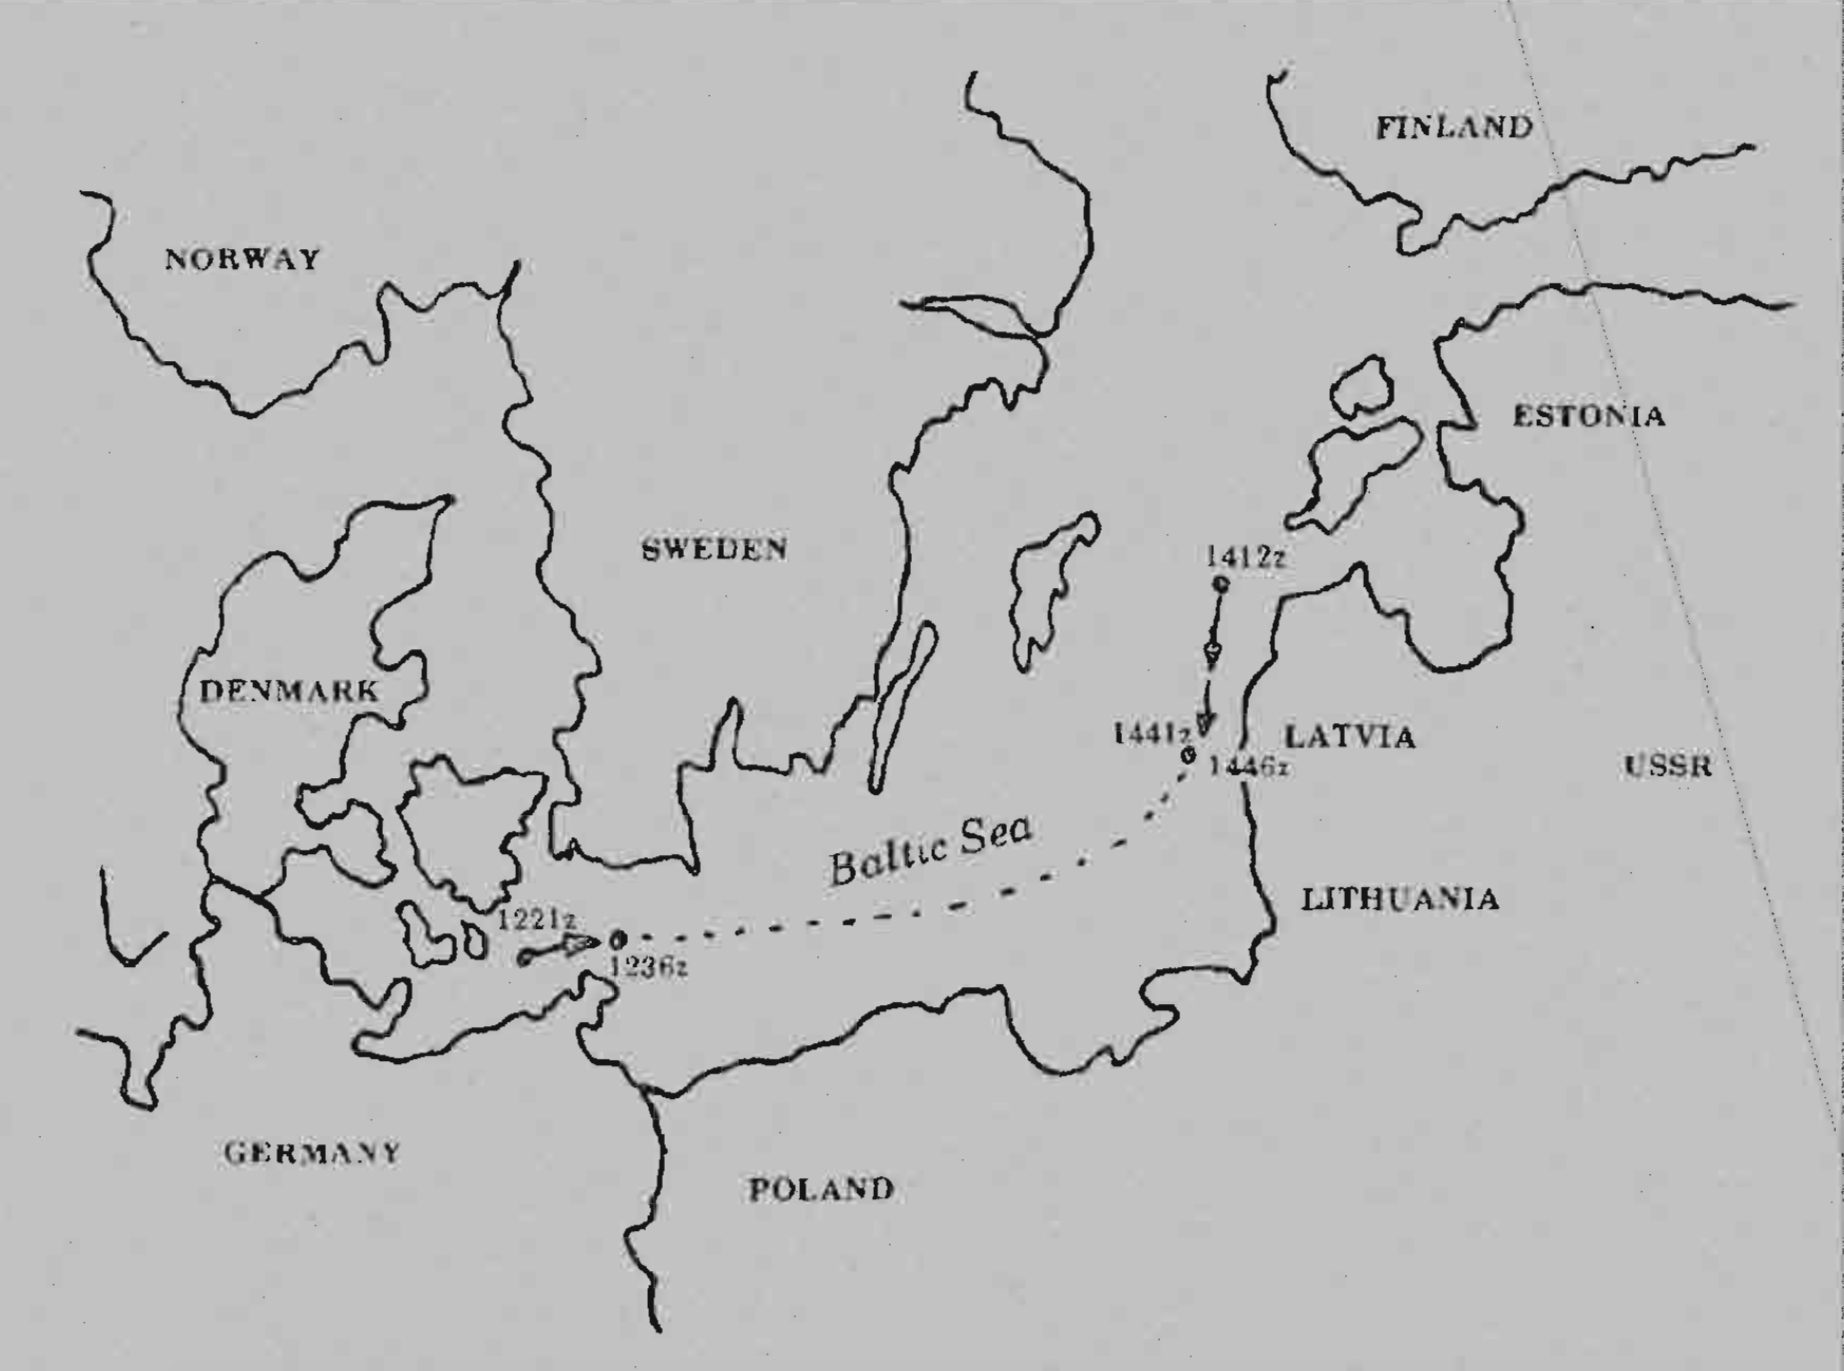
\includegraphics[scale=0.45]{baltic-flight-path.png}
\caption{USN PB4Y2 Flight Path}
\label{baltic-flight-path}
\end{figure}

Meanwhile, The United States knew that they hadn't lost a B-29, and that it probably hadn't ended up in Soviet airspace, but the Privateer in question \emph{had} been performing a questionably legal reconnaissance mission when it was shot down. Though the US was likely correct that it never flew over Latvia, it certainly got as close as it needed to in order to gather the necessary intelligence about Soviet military installations on the coast. No traditional boundaries were violated, but a repurposed Navy privateer loaded down with electronic reconnaissance equipment flying close to Latvia looked, to use a less technical term, shady. Yet based on the initial exchange of diplomatic protests, neither side was inclined to magnify the issue if they could avoid it.

The American press had no such reservations. \emph{Washington Post} columnist Walter Lippmann wrote that it could not have been ``a local incident brought on by a local commander but [rather] that it was an act of Soviet policy. The known facts indicate that Soviet intelligence \textelp{} believed it was carrying important electronic equipment and that orders were given to the Soviet fighter command to intercept it.''\footcite{lippmann_baltic_1950} He speculates that there is no way the plane could have violated Soviet airspace, because wreckage would have been recovered, the plane was too slow, and no commander would have sent it on such a dangerous mission intentionally. ``If, when, and as the American command were reconnoitering the Soviet military establishments on the Baltic coast,'' Lippmann wrote, ``it would use a plane of a wholly different type.''\footcite{lippmann_baltic_1950}

A newspaper columnist is not a policymaker, but his argument is likely reflective of the general attitude towards espionage of this sort at the time. That attitude is striking. Of course we do these things, we just do them \emph{better} than that---and if we had been doing the thing that the Soviets claimed we were, then it would have been justified of them to shoot us down. ``Baltic Plane Mystery,'' a \emph{Post} article written a few days later, is almost sympathetic to the Soviet commanders. ``Electronics make the old delimitations for border coastal flights ridiculous. A plane flying on a course perfectly legal by standards accepted today might still be engaged in reconnaissance of the first importance that an unfriendly power would try to frustrate.''\footcite{childs_baltic_1950} This is true, both in terms of the mission itself and the technological environment, but he goes even further. ``The only sound and safe assumption is that the Russians have a thorough and far-reaching espionage system. And at the same time we must hope that our system, and particularly on the side of counterespionage, is effective.'' Even the press, though outraged at the loss of American life, seems have taken it as a given that this kind of espionage is necessary, and expected from both sides.

The most important consequence of the Baltic Incident was not diplomatic. As a direct result of the shootdown, President Truman, who until that point was largely uninformed about these missions, ordered a thirty-day halt to all reconnaissance flights. In that time, his office came up with an operating procedure that would balance the strategic need for reconnaissance with its potential diplomatic volatility.\footcite[p.~41]{farquhar_aerial_2015} The resulting memo from the Joint Chiefs of Staff created, with Truman's approval, the Special Electronic Airborne Search Project (SESP), which set clear delineations of responsibility between Navy and Air Force reconnaissance, and established executive responsibility for approving the missions.

Farquhar cites this as a landmark moment in the history of aerial reconnaissance. ``No longer would ferret operations be conducted ad hoc by the military services;'' he writes, ''from 1950 onward, reconnaissance operations attracted Presidential attention and played a significant role in shaping U.S. foreign policy.''\footcite[p.~42]{farquhar_aerial_2015} The strict procedures that SESP established were crafted to avoid the risk of escalation, while still explicitly acknowledging the ``serious disadvantages accruing to the United States if the cessation of these operations were to be extended over an excessively long period.''\footcite{bradley_memorandum_1950} But the SESP procedures also contain a curious provision: ``Flights will not be made closer than twenty miles to the USSR or USSR- or satellite-controlled territory.''\footcite{bradley_memorandum_1950} This rule would not be followed.

\subsection{Routine resolution}
Between the shootdown of the Navy Privateer in 1950 and the famous U-2 shootdown in 1960, the United States lost nine more aircraft to Soviet air defenses. While I do not have the space to analyze each one in the same level of detail, I can demonstrate how the general attitudes displayed in response to the Baltic Incident became normalized. In each of the incidents listed, the pattern is the same---each side releases dueling statements of protest, and situation continues more or less as before.

Very briefly, here are the next few peacetime reconnaissance shoowdowns whose diplomatic consequences Farquhar analyzes. A B-29 that went missing on October 7, 1952 hit the front page of the \emph{New York Times} two days later. This mission is on Peterson's list as a ferret flight. Farquhar notes that the incident happened during the US election season and that the media thought the attack was intended to lower American prestige, but he does not mention any diplomatic consequences.\footcite[p.~43-44]{farquhar_aerial_2015} The official US response, however, is preserved on the State Department website. As with the Baltic Incident, the US simply demanded that the Soviets pay for the plane and return any survivors.\footcite{the_new_york_times_u.s._1952} Two more shootdowns in March 1953---one involving and American F–84 Thunderjet and the other an RAF Lincoln bomber---actually resulted in conciliatory tones from both sides, including apparently a secret meeting to reduce aerial tensions ``of which little is known''.\footcite[p.~45]{farquhar_aerial_2015}

In another incident on July 29, 1953, a B-50 (reconnaissance flight) was shot down over the Sea of Japan. The United States protested, and in response the Soviets counter-protested an alleged American shootdown of a Soviet passenger plane. Despite press outrage, no further action was taken.\footcite[p.~47]{farquhar_aerial_2015} A September 4, 1954 shootdown of a Navy P2V Neptune actually led to a call by one US Senator to break off diplomatic ties with the Soviet Union. ``Just another note from our State Department to the Kremlin hierarchy will not impress these uncivilized rulers \textelp{} that this new attack upon an American plane confirms Communist arrogance and aggressiveness to a point where the breaking of diplomatic relations is justified.''\footcite{the_associated_press_ending_1954} Instead of a harsher punishment, Eisenhower brought it to the UN with the full knowledge that even if an unfavorable decision was reached, it would be vetoed by the Soviets. Although the move was entirely symbolic, it signaled Eisenhower's ability to resist the calls for harsher action while still placating the American public.\footcite[p.~47]{farquhar_aerial_2015}

I do not wish to belabor the point, so suffice to say that Farquhar's conclusion is that after this moment in 1954, the resolution of these incidents became less tense. ``International incidents posed by shoot downs of reconnaissance aircraft still acted as a barrier in the path of d\'etente; but, by late 1954, overriding strategic concerns dictated a move toward breaking the cycle of hostility.''\footcite[p.~49]{farquhar_aerial_2015} In terms of media coverage, and diplomatic significance, no shootdown that followed would require more significant consequences than the ones that had already happened.

% Valentino: Just produce a table here

There is one incident in the period between 1950-1954 that does not fit the broader pattern. On November 20, 1951, an American C-47 transport was forced down in Hungary. This incident is omitted from Peterson's list because, despite Soviet cries of ``spies and saboteurs,'' there is no evidence that it was a reconnaissance flight.\footnote{It also wasn't exactly shot down so much as forced to land.} Of all the cases that Farquhar examines, this is the only one that provokes a sustained diplomatic response from the United States---and it is the only case where the plane in question definitively carried no espionage equipment. While the ferret flights were perfectly calibrated to fit as much radio surveillance equipment as possible, the only evidence of espionage that the Soviets were able to produce from the C-47---a plane that they recovered intact---was a portable radio, two extra parachutes, and some packets of warm blankets.\footcite{the_united_press_soviet_1951}

I contend that the lack of espionage equipment is precisely the reason the United States made a sustained public effort to recover the four airmen, which is something that almost never happened with these flights.\footnote{While some of the flights were shot down overseas, making recovery difficult, I am referring here to situations where the US was aware that the Soviets likely held their airmen in captivity and still made little effort to get them back.} Farquhar summarizes the American answer to this incident like this: ``Responding to the press attention, the Truman Administration acted swiftly, attempting to gain the fliers release through diplomatic pressure. The President ordered the Hungarian consulates in New York and Cleveland closed and banned private travel to the country. Legislatively, Truman asked Congress to pass a \$100 million Mutual Security Act to aid `selected persons residing in Soviet bloc states or refugees who wanted to form armed units' in opposition to Communism.''\footcite[p.~43]{farquhar_aerial_2015} Truman immediately took action against material Hungarian interests in the United States and threatened to empower \emph{armed dissidents} if the prisoners were not released. The contrast between this response and the one from just a year prior, when the US demanded ``a prompt and thorough investigation'' of the Baltic Incident, is stark.

We also know that the United States conducted many more overflights than the failed ones that are listed here, using a wide variety of retrofitted planes. In 2001, the Air Force held a symposium honoring and recollecting the pilots who flew the overflights on Soviet territory in the early Cold War, an effort in which they were joined by the British in 1954.\footcite[p.~v]{hall_early_2003} Many of the presenters spoke about entire reconnaissance projects that apparently didn't even register diplomatically. Project Heart Throb, which outfitted RB-57s with surveillance equipment, flew anywhere from 15 to 19 missions over Eastern Europe from 1955 to 1956, in the recollection of Gerald E. Cooke, a Air Force pilot assigned to the project.\footcite[p.~194]{hall_early_2003} Another project from around the same time, Slick Chick, set up F-100 jets with rapid-fire 20mm cameras. The pilot who presented about this project at the symposium, Cecil Rigby, personally flew two such missions. Though he was attempting to recall highly classified events from 50 years prior, he estimated that there were six Slick Chick missions total.\footcite[p.~176]{hall_early_2003}

The USSR knew about these overflights, which were tracked by radar and often chased by MiG fighters. Unlike some of the flights that were shot down, these overflights were clear violation of their territorial sovereignty. We will likely never know exactly how many such missions were flown. The Truman and Eisenhower administrations were shockingly bad at recovering the pilots who were held as POWs by the Soviets. Dino Brugioni, a senior CIA officer involved in the aerial imagery program, paints a grim picture of the institutional accountability involved when the flights went bad. In meetings between the State department and high-level Soviet diplomats, the subject of captured pilots ``was broached only perfunctorily in relation to other things being discussed.''\footcite[p.~72]{brugioni_eyes_2010} Some family remembers of lost airmen received posthumous awards, but most simply received his personal effects and no explanation. ``And because these were secret missions conducted by a field command,'' he writes, ``a change of field commander meant that the fate of the men was soon forgotten.''\footcite[p.~72]{brugioni_eyes_2010} With missions so secret that we abandoned the men who flew them, we can have no expectation of finding a complete record today.

Even without a complete list of flights, it is clear that the territorial boundaries of the USSR were routinely violated to generate critical intelligence for NATO powers in an early, relatively volatile stage of the Cold War. As time went on these flights appear to have become more acceptable, not less. Diplomats of both nations were, as a matter of policy, able to paper over these issues in service of moving on to other matters. When the shootdown had unavoidable diplomatic consequences---which happened when it was well-publicized---then they exchanged the necessary diplomatic cables and engaged in the requisite saber rattling. These incidents undoubtedly altered the climate of Cold War diplomacy, but the fact remains that in 10 years of reconnaissance, the only thing the Soviets did to keep the United States from conducting these incredibly provocative reconnaissance flights was to shoot them down.

% Valentino: Can you talk about other ways the Sovierts might have responded. What other kinds of actions might have seemed reasonable under different norms? Maybe give an example of a Soviet response to something apparently similar on its face, but clearly out of the espionage domain, so the response was much harsher.

\section{Civilian spy flights}
\subsection{Project Aquatone}
While Eisenhower was able to defuse some of the tension around the military reconnaissance flights, even the most aggressive overflights could only hope to skirt the borders of Soviet territory. The United States couldn't just send a B-50 over Moscow. What US intelligence-gathering capabilities needed was some way of photographing suspicious installations deep within Russia while still being able to claim the same benefit-of-the-doubt status that prevented even the most contentious overflights from escalating into a larger conflict. What they needed was a spy plane.

The key feature of a spy plane is that it is designed to be minimally provocative. As detailed earlier, any plane can be retrofitted with cameras or radios that allow it to perform useful reconnaissance functions. What differentiates a spy plane is that there can can be no doubt that it is being used for anything else. For the spy plane to serve its intended purpose as a minimally provocative agent of espionage then, two things must be true: its operation must be understood by adversaries to be non-military, and that distinction must meaningfully alter their threat perception and associated response. To build such a aircraft, Eisenhower approved Project Aquatone, the code name for the creation of the U-2.

From its conception, the U-2 was purpose-built to be read as a civilian aircraft. Eisenhower required that the pilots of U-2 aircraft be CIA employees, specifically forbidding uniformed Air Force officers.\footcite[p.~33, Though many of the pilots did have Air Force backgrounds.]{lindgren_trust_2000} This is also the reason that that the CIA had operational control of the program over the Air Force. ``I want this whole thing to be a civilian operation,'' Eisenhower wrote to settle an operational dispute between the two departments. ``If uniformed personnel of the armed services of the United States fly over Russia, it is an act of war---legally---and I don't want any part of it.''\footcite[p.~60. The original source for this quote is an \emph{OSA History} that requires codeword clearance. It is quoted here by the History Staff of the CIA.]{pedlow_central_1992} This also allowed the United States to ``truthfully deny,'' in the phrasing of the CIA, that any US ``military planes'' had flown over the USSR---which they had to do when the inevitable Soviet protest notes were filed after U-2 overflights began in 1956.\footcite[p.~109]{pedlow_central_1992}

It is worth considering for a second how having the CIA run the program---ostensibly for the purpose of deception---changes the nature of the program itself. If the only goal here had been to achieve a level of plausible deniability in the event of a shootdown, then not wearing an Air Force uniform during the mission seems like it would have been sufficient. The ``weather reconnaissance'' excuse had even been used before with the ferret flights.\footcite[p.~45]{farquhar_aerial_2015} At the highest levels of American government, policymakers didn't just want to pretend that Aquatone was a civilian operation, they wanted it to \emph{be} a civilian operation---even if the planned NASA weather-craft cover didn't hold. ``It is of utmost importance to differentiate in our minds, and to cause the Russians to differentiate in theirs, between Aquatone-type operations and reconnaissance by military aircraft'' reads a top-secret CIA memo from 1956.\footcite[p.~1]{miller_suggestions_1956} Both halves of that are equally important. The Russians must believe that these operations are peacetime civilian operations, and they must be correct about it.

The United States was aware how provocative these reconnaissance flights might be, and Eisenhower was always concerned, correctly, about ``the terrible propaganda impact that would be occasioned if a reconnaissance plane were to fail.''\footcite[p.~162]{pedlow_central_1992} But he was also under tremendous political pressure to learn more about the Soviet missile program, as right-wing senators hyped up fears of a so-called ``missile gap,'' concerned that Soviet ballistic missile capabilities were advancing faster than our own.\footcite[Fears of this missile gap quickly followed earlier fears of a ``bomber gap,'' which ironically the U-2 had been critical in disproving.]{licklider_missile_1970} Starting in 1958, the American administration ordered a drastic decrease in the number of overflights.\footcite[p.~51]{powers_operation_2004}

It turned out however, that the Soviets opted to lodge their diplomatic protests privately, and soon they stopped protesting them at all.\footcite[p.~42]{lindgren_trust_2000} The Eisenhower administration fatally misinterpreted this sign. ``It is one of the many unfortunate aspects of the high degree of secrecy surrounding Moscow's actions,'' imagery analyst David Lindgren writes, ``that the United States never understood the how angered and frustrated Soviet leaders were made by the U-2 overflights.''\footcite[p.~52]{lindgren_trust_2000} What does their frustration say about the spy plane's civilian image and its ability to prevent conflict escalation? As with the military reconnaissance flights, that question can be answered by investigating the maximal case. Fortunately, there is a single moment that is unquestionably the most significant diplomatic drama to emerge from a Cold War spy plane mission: the shootdown of Gary Powers, best known as the ``U-2 Incident.''

\subsection{The U-2 Incident}
On the morning of May 1, 1960, Soviet Air Defense forces detected a high-altitude aircraft flying over Soviet Tajikistan. Though they were were not yet able to conclusively identify it, the foreign aircraft was an American U-2 spy plane performing an reconnaissance overflight of the USSR---at a time when the Soviets were deeply embarrassed by their inability to prevent such flights.\footcite{orlov_u-2_2007} A previous U-2 overflight on April 9, less than a month prior, had lasted a full six hours and the aftermath caused an upheaval in the Soviet military. Leadership ordered an investigative commission to root out the shortcomings of the Air Force and Air Defense agencies, and a series of charts were drawn up anticipating the routes of future U-2 flights. The next time one came through, the Soviets were absolutely determined to shoot it down.

\begin{figure}
\centering
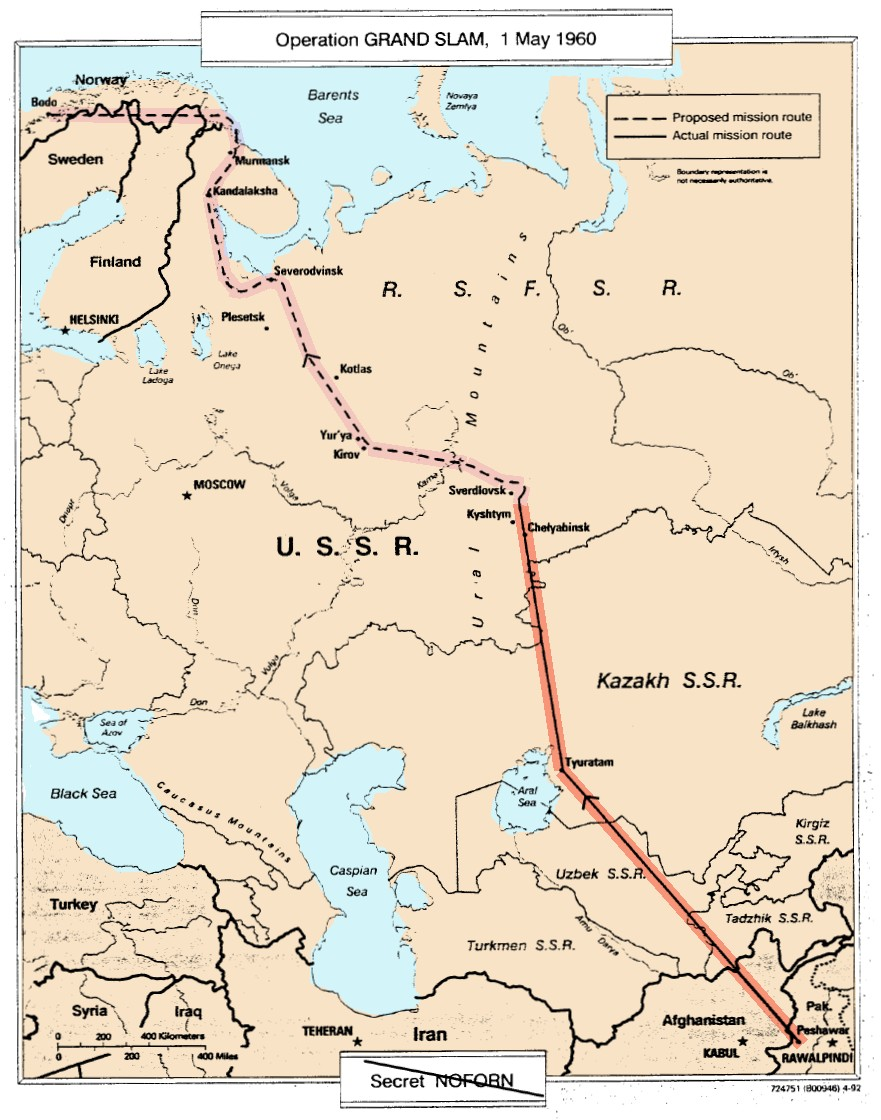
\includegraphics[scale=0.3]{powers-flight-path.jpg}
\caption{Operation Grand Slam Flight Path}
\label{powers-flight-path}
\end{figure}

Though better prepared, the Soviets still proved unable to immediately stop the flight on May \nth{1}. A missile battalion in the plane's path was not on alert duty. Armed fighter aircraft were in the wrong positions. A frantic attempt to have another fighter plane literally ram it out of the sky was scrapped when the pilot failed to make visual contact.\footcite{orlov_u-2_2007} The highest possible levels of Soviet leadership were actively involved with the mission as it was taking place. A Soviet Colonel in the USSR Air Defense later recalled that Khrushchev ``clearly viewed the violation of their nation's skies by a foreign reconnaissance aircraft on the day of a Soviet national holiday, and just two weeks before a summit conference in Paris, as a political provocation.'' \footcite{orlov_u-2_2007}

Why did the generally cautious Eisenhower authorize two overflights in such close proximity to a crucial summit? For one, the secrecy of the program worked against him. Eisenhower was not willing to make the U-2 program public, so he couldn't convince his critics that he had intelligence of extremely high quality that no such missile gap existed, because to reveal the existence of his aerial photography would prompt questions about its origins.\footcite[p.~51]{lindgren_trust_2000} And the missions had been such a tremendous success that his reluctance to authorize more overflights grated his staff, especially the influential Director of Central Intelligence (DCI) Allen Dulles.\footcite[p.~354]{brugioni_eyes_2010}

Another crucial factor emboldened Eisenhower and his team---most of whom, like Dulles, were much more enthusiastic about overflights than he was---to conduct that second mission. The USSR had been aware of the April 9 flight, and the United States \emph{knew} that they were aware of it, thanks to an onboard computer that had detected the Soviet tracking from the beginnings of the operation.\footcite{pedlow_central_1992} From the perspective of the American administration, the lack of a protest note after the last flight was a sign that the USSR was not particularly offended by the overflights. Interpreting Soviet silence on this issue as encouraging was a severe miscalculation by the Americans. After years of bluster about the superiority of Soviet military forces, Khrushchev was not about to admit that his Air Defense could not shoot an unarmed spy plane flying deep into his homeland. They couldn't do anything about it, and they refused to admit that by simply lodging a protest.\footcite[p.~59]{powers_operation_2004} This was a military shame, and it was going to be resolved with a missile.

Almost four hours into the spy plane's flight on May 1, pilot Francis Gary Powers felt a dull ``thump'' and ``a tremendous orange flash lit the cockpit and sky'' as a Soviet surface-to-air (SAM) missile exploded behind him, ripping the wings off his plane and sending it into a tailspin.\footcite[p.~61]{powers_operation_2004} His subsequent crash and capture by the Soviet military became an immediate international incident. Three days after NASA quietly reported that they had lost a U-2 type weather reconnaissance plane, Khrushchev announced that the USSR had shot down an American plane that had flown into their airspace, which he called ``an aggressive provocation aimed at wrecking the Summit Conference.''\footcite[p.~112]{powers_operation_2004} Once Khrushchev gleefully debunked the resulting American cover story by revealing that they had taken Powers alive, Eisenhower came clean in a Press Conference where he memorably declared that espionage was a ``a distasteful but vital necessity'' to prevent another attack like Pearl Harbor.\footcite{eisenhower_news_1960}

Publicly, the USSR was not ready to accept that US overflights of its were a ``distasteful but vital necessity.'' The Four Powers summit in Paris was disastrous. Khrushchev launched into an angry rant on the first day and stormed out, immediately squashing any hope that pressing issues like the fate of West Berlin would be resolved there. He also canceled a planned visit by Eisenhower to the USSR that was scheduled to take place the next month. A contemporary newsreel about the conference said that ``in the course of two hours, Khrushchev brought US-Soviet relations to their lowest point since the end of World War II.''\footcite{universal_studios_summit_1960}
% The contrast between the severity of response Khrushchev wanted to portray publicly and what the USSR actually did is highlighted by his own son Sergei, who edited and annotated the 2007 edition with notes featuring additional context for his father's statements.

\section{Espionage in the open skies}
\subsection{Minimal consequences with maxmimal noise}
The U-2 Incident is often cited as a major failure of the Eisenhower administration. In the classical telling, it significantly worsened US-Soviet relations at time when it seemed like lasting peace might be possible. I disagree. Instead, I argue that it should be understood as an embarrassing but otherwise typical failure of an intelligence operation, one consistent with the minimal consequences typically applied to espionage.

No one disputes that the collapse of the Paris Summit is directly attributable to the Gary Powers shootdown but, frankly, summits just aren't that important. From 1953 to the end of the Cold War in 1991, there were 23 total US-USSR summits.\footcite{fain_chronology_2011} The main issue that did not get resolved in 1960 was the status of Berlin. It also did not get resolved at the next summit in 1961, a comparatively warmer affair between Khrushchev and Eisenhower's successor, John F. Kennedy. If the worst that happened because of the U-2 incident was an unproductive summit meeting, then that's a relatively minor punishment. With the late rollout of the captured pilot, the dramatic scene at the summit, and canceling Eisenhower's visit, Khrushchev publicly embarrassed the United States without meaningfully altering Soviet policy towards it.

What would a major punishment have looked like? One proportional response that Khrushchev could have considered is to force the issue on regional air bases. Since the US was using nearby bases to launch invasive reconnaissance missions, it stands to reason that the Soviets could have demanded that they either close some of them or agree to halt surveillance flights. This likely would have involved some sort of trade, but it is not an unreasonable hypothetical. The Soviets were incredibly preoccupied with removing the forward-deployed Jupiter missiles from Turkey---missiles who bases were also safely in NATO territory, but whose presence arguably did less damage to the Soviet military posture than American intelligence about the missile gap; missiles which became a central bargaining chip in the Cuban Missile Crisis. They simply did not have the same level of interest in curtailing reconnaissance flights. That both sides of the Cold War had strong incentives to avoid military escalation is well-documented, but at least threatening military retaliation for launching provocative military operations would not seem to have been out of place.

While I argue that the response to the U-2 flight was within the reasonable bounds for espionage, I acknowledge that it was still unprecedented in the context of reconnaissance flights. There are a number of reasonable explanations for why the U-2 shootdown escalated. Partially the Soviets felt humiliated by a technology for which they had no countermeasures, and the uniquely insulting way the overflights flew deep into Soviet territory. Eisenhower thought that Khrushchev might have been looking for an excuse to cancel his visit to Russia.\footcite[p.~555]{eisenhower_waging_1965}. Others in his administration believed that the U-2 Incident was an excuse to justify a turn towards an intensification of hostilities that had already been decided by hard-liners in the Kremlin.\footcite[p.~328]{kistiakowsky_scientist_1976}

Most scholars who study this period argue that the cumulative tension created by these flights contributed to an overall chilly tone in US-Soviet relations. Farquhar, for instance, calls this the ``cycle of hostility,'' in which the series of aerial incidents increased suspicions of military buildup on both sides, leading to even more aerial incidents as both powers attempted to verify their suspicions.\footcite[p.~43]{farquhar_aerial_2015} While it's true that the there were a lot of aerial incidents, it is not at all clear how this affected any other aspect of US-Soviet diplomacy. I can't definitively say that there isn't some diplomatic issue that would have gotten resolved at a summit absent these reconnaissance flights, but I can't find an obvious one either.

Consider the period of time over which these flights took place. If aerial reconnaissance had been anything more than a lingering issue, then it would have to have been resolved in some way before 1960. The US-Soviet relationship saw huge shifts, including periods of optimism, over the 11 years this was going on until the U-2 incident. Hundreds of flights taking place in contentious territory, many of them purposefully violating Soviet boundaries, some of them shot down, and the worst that happened in that whole time was a bad summit meeting, after which the flights continued on almost as before. Even with soldiers' lives on the line, both sides were so willing to contain the issue that many of the airmen never saw their families again.

\subsection{The U-2 after Powers}
When the US really needed some particular intelligence that only an overflight could provide, the diplomatic consequences that the USSR had imposed were not sufficient to discourage it. Two months to the day after Powers was shot down, July 1, 1960, a Soviet MiG-19 opened fire on an American RB-47H and captured the plane's navigator and the co-pilot. While Powers was serving a 10-year sentence in Soviet prison, the two airmen were returned to the US less than six months later with only mild fanfare shortly after John F. Kennedy's inauguration, in early February, 1961. Khrushchev wrote in his memoir that he wanted to continue ``our general line of peaceful coexistence'' and cites the resolution of this incident as an example of such, where the US was forced to make a formal request for the return of the airmen.\footcite[p.~256-257]{khrushchev_memoirs_2007} The only relevant concessions the US made in return were to announce the discontinuation of its U-2 overflights (which Kennedy was already committed to) and to not make an issue of the illegal detention of the pilots.\footcite{time_cold_1961} They simply took the necessary immediate countermeasures, and shot down the planes that they could. Just as with traditional espionage, the countermeasures did not punish the attempt.

Until the day he died, Khrushchev greatly exaggerated the lasting effect of the U-2 Incident. He writes in his memoir that ``the commander of American forces in West Germany gave the order not to fly any closer than 50 kilometers from the border between East and West Germany. And no more incidents of that kind occurred.''\footcite[p.~256]{khrushchev_memoirs_2007} His son Sergei, who annotated the memoir, admits that this statement is false: ``In practice such incidents occurred again from 1961 onward, but instead of the U-2 the Americans now used various types of Phantom or SR-71.''\footcite[p.~258]{khrushchev_memoirs_2007} On at least two occasions after the U-2 Incident, an American overflight crossed over into Soviet territory and the Soviets responded with... a diplomatic protest. The US quickly apologized, and that was that.\footcite{orlov_u-2_2007}

The U-2 did not disappear after the Powers flight. A recently declassified CIA report details the many locations in which the CIA deployed the U-2 to gather intelligence after May 1, 1960, including China, India, Indonesia, Thailand, Tibet, Laos, North Vietnam, and Venezuela. Lyndon Johnson even clarified that his predecessor's order to end U-2 flights over the Soviet Bloc was not indefinitely binding---it was valid only until countermanded.\footcite[p.~195]{pedlow_central_1992} As it turned out, it  never became necessary to resume Soviet Bloc overflights because satellite photo-reconnaissance served a similar purpose. U-2 overflights were rendered mostly obsolete.

I say mostly because there is one use-case in which satellites will likely never displace aerial photo-reconnaissance---a situation like the Cuban Missile Crisis, where events are so time-sensitive that intelligence is needed in a matter of hours. On October 15, 1962, U-2 photography revealed that the Soviet Union was assembling missile in Cuba that were capable of carrying nuclear warheads. As the crisis unfolded, the United States continued to send U-2 planes over Cuba in order to maintain a close watch on the development of the missile sites. Kennedy's team decided that if a U-2 were to be shot down, the most likely SAM site would be immediately fired upon.\footcite[p.~217]{caro_passage_2013} Then, on October 27, it happened---a U-2 was shot down flying over Cuba and the pilot was killed. Kennedy flinched; he had just sent Khrushchev an offer that might lead to peace, and he didn't want to jeopardize it. Against the advice of the administration hard-liners, including Vice President Johnson, Kennedy refused to authorize the strike against the Cuban SAM site.\footcite[p.~220]{caro_passage_2013} The next day, Khrushchev agreed, and the Cuban Missile Crisis ended with only a single casualty---the U-2 pilot, Major Rudolph Anderson.

As his title indicates, Rudolph Anderson was an Air Force Officer, not a member of the CIA. During the crisis, the President transferred control of Cuban U-2 reconnaissance to the Air Force, and authorized it to fly as many missions as necessary over the island.\footcite[p.~208-209]{pedlow_central_1992} Khrushchev does not say much about the Cuban U-2 in his writing, but he is very clear on one point: he did not order the strike, and was worried that Kennedy ``might not be able to absorb this blow.''\footcite[p.~338]{khrushchev_memoirs_2007} Shooting down an American aircraft risked escalation, and that was not something that Khrushchev wanted. This was the second time in history that Soviet forces had shot down a U-2 plane---but even though the spy plane flying over Cuban airspace and pilot by an Air Force Major, it was the Soviets who were worried that shooting it down had been an unnecessary, potentially fatal aggressive act.

\subsection{Bridge of spies}
The role that the U-2 played during the Cold War perfectly mirrors the traditional consequences for espionage because United States succeeded in applying the norms of espionage to a new device. Eisenhower's insistence on having Project Aquatone managed by the CIA had the intended effect: the spy plane was, in story as well as fact, a civilian intelligence operation.

The one time an operation went truly bad, it still played by the rules of the game. Powers opted against using his suicide capsule, but the macabre truth about the U-2 is that pilots weren't supposed to survive a crash at all. The United States originally went with the weather craft story because Eisenhower had been assured that Gary Powers could not possibly be alive to tell the Russians the truth.\footcite[p.~35]{lindgren_trust_2000} When Powers confessed to his Soviet captors, he told them, correctly, that he was a civilian pilot with the CIA. His cover had been blown, but underneath it he was still a spy, and in pretty much all respects he and the U-2 were treated accordingly.

Both heads of state made clear in their writings that they considered Powers to be spy. On capturing Gary Powers, Khrushchev wrote ``This was a hostile act by the leaders of the U.S. government, and they made no attempt to conceal it. They didn't think we had the capability of \textelp{} acquiring irrefutable proof that the United States was using methods that were impermissible in peacetime.''\footcite[p.~239]{khrushchev_memoirs_2007} Sergei's annotations once again contradict his father's claim that these methods were impermissible; more than forty American reconnaissance aircraft were shot down by the USSR during the Cold War. As is often the case with espionage, Khrushchev wanted to make it seem like he was standing up for the integrity of the Soviet state without endangering the espionage equilibrium.

Eisenhower, always an insightful thinker on issues of intelligence, understood that beneath the grandstanding, the fundamentals of international espionage applied. In his own words:

\begin{quote}
	Furthermore, it seemed to me that Mr. Khrushchev's outbursts were hypnotizing the world with a passionate but highly distoreted presentation of one particular phase of international espionage. His government had been so notoriously involved in spying, especially in the United States, as to dwarf our activities, but by separating this particular type of espionage from all others he hoped to make convincing his charge of ``warmongering.'' To claim that because the equipment employed was an airplane with a camera, and therefore provocative of war, was plain silly, and I felt it necessary that the matter be put in perspective. \\

	The real issue at stake was not the fact that both sides conducted intelligence activities, but rather that the conduct and announced intentions of the Communists created the necessity for such clandestine maneuvers. As a consequence, the West---more specifically the Untied States as the major military power of the West---had to maintain constantly the capacity to detect any possible prelude to an infinitely more destructive Pearl Harbor.\footcite[p.~551]{eisenhower_waging_1965}
\end{quote}
The next chapter goes in depth on how the fear of a nuclear Pearl Harbor affected the entire American intelligence strategy, but even in the limited context of the spy plane, it is clear that Eisenhower deployed espionage to de-escalatory effect. Khrushchev had convinced the world that the Soviet missile capabilities were far more advanced than they actually were. Eisenhower was under tremendous pressure from the public, Republicans in Congress, and even his own staff to increase the Defense budget. The only thing standing between Eisenhower and an accelerated arms race were detailed photo-reconnaissance reports from the U-2, that showed the Soviets were developmentally far behind what their public statements suggested.

The peaceful uses of aerial reconnaissance were formalized at the end of the Cold War, when members of NATO and the Warsaw Pact signed the ``Treaty on Open Skies,'' which established guidelines for unarmed aerial surveillance flights in the spirit of open information and de-escalation.\footcite{organization_for_security_and_co-operation_in_europe_treaty_1992} This was almost identical to the concept first suggested by Eisenhower in 1955.\footcite{center_for_arms_control_and_non-proliferation_fact_2017} With certain restrictions, the kind of flight that altered the course of the Cold War is now officially routine and permissible.

In February 1962, Francis Gary Powers walked across a bridge into West Berlin at the same time as Russian Colonel Rudolph Abel, an American prisoner. Powers' father had suggested to the State Department that they might be traded, spy for a spy.\footcite[p.~239]{powers_operation_2004} ``This,'' Eisenhower wrote, ``was a tacit admission by Khrushchev that our `outrageous' U-2 pilots have their opposite numbers operating within the borders of this country.''\footcite[p.~558]{eisenhower_waging_1965} The Powers flight and Project Aquatone channel the norms of espionage in one final, but crucial respect; their strategic value easily outweighed the consequences of being caught. No one understood this better than President Eisenhower, who, when asked about the wisdom of the U-2 flights, would reply: ``Would you be ready to give back all of the information we secured from our U-2 flights over Russia if there had been no disaster to one of our planes in Russia?'' In his telling, he never received an affirmative response.\footcite[p.~559]{eisenhower_waging_1965}

\newpage
\printbibliography[heading=subbibliography]

\end{refsegment}
\end{document}
